\documentclass[11pt,a4paper]{article}

\usepackage[utf8]{inputenc}
\usepackage[T1]{fontenc}
\usepackage{amsmath,amssymb}
\usepackage{geometry}
\usepackage{booktabs}
\usepackage{listings}
\usepackage{pgfplots}
\usepackage[colorlinks=true,linkcolor=blue,citecolor=blue,urlcolor=blue]{hyperref}

\geometry{left=2.5cm,right=2.5cm,top=2.5cm,bottom=2.5cm}
\pgfplotsset{compat=1.18}

\lstset{
  basicstyle=\ttfamily\small,
  breaklines=true,
  frame=single,
  numbers=left,
  numberstyle=\tiny,
  tabsize=2
}

\title{\textbf{NRR-Coupled (cp) v2: Coupled State Update Under Candidate Dependencies}}
\author{Kei Saito\\Independent Researcher, Japan\\\texttt{kei.saito.research@gmail.com}}
\date{February 2026\\[0.5em]\textit{Part of the Non-Resolution Reasoning (NRR) research program.}}

\begin{document}
\maketitle

\begin{center}
\textcopyright\ 2026 Kei Saito. Licensed under CC BY 4.0.\\
\url{https://creativecommons.org/licenses/by/4.0/}
\end{center}

\begin{abstract}
NRR-Transfer defines an uncoupled state-update interface for independent candidates: the LLM selects a directional operator (\(\sigma\)/\(\delta\)) and target, and the client executes deterministic updates. This paper defines NRR-Coupled (cp), a coupled extension for dependent-candidate conditions. The interface contract is unchanged on the LLM side; only client propagation is extended. We specify the coupled update law, complexity bounds, applicability and failure conditions, and a simulation-first evaluation protocol. The main experiment is deterministic simulation (no API calls): fixed operator sequences are applied to uncoupled and coupled systems under three dependency conditions (dependent / independent / mismatch), with \(\beta\in\{0.1,0.3,0.5\}\). Results show small positive utility gains in dependent conditions, exact uncoupled/coupled equivalence under independent conditions, and elevated oscillation under stronger coupling. The evidence supports a conditional claim: cp is useful when dependencies are informative and coupling is controlled, but it is not universally superior.
\end{abstract}

\noindent\textbf{Keywords:} NRR-Coupled, coupled update, dependency propagation, simulation evaluation, falsifiable protocol

\section{Introduction}
LLM APIs are stateless across calls, but many systems require persistent state updates over candidate sets. NRR-Transfer addressed this under independent-candidate assumptions. This paper introduces \textbf{NRR-Coupled (cp)} for conditions where candidates are dependent.

NRR is not an anti-LLM framework.
NRR does not replace standard LLM use.
NRR optimizes when to commit and when to defer, under explicit conditions.

\textbf{Claim boundary.}
Transfer covers independent-candidate conditions. cp covers dependent-candidate conditions. The uncoupled baseline is inherited from Transfer and is not redefined.

\textbf{Design constraint (first hypothesis).}
The LLM-side interface is unchanged: emit \((\sigma/\delta,\;\text{target})\). cp changes only client-side propagation. If this contract fails in deployment, record `TRANSFER\_PRINCIPLES\_REEVAL\_REQUIRED=true` and continue cp-side diagnosis.

\textbf{Experiment direction.}
The main evaluation is simulation-first (no API): identical pre-defined operator sequences are injected into uncoupled and coupled clients to isolate update-law effects.

Series Consistency Statement: Unsupported interpretations are never injected at a fixed evidence state. Hypothesis-set expansion is evidence-gated, and unobserved possibilities remain unresolved. Evidence in this paper is restricted to explicit input, fixed operator streams, and declared dependency matrices.

\section{State and Coupled Update Rule}
Let \(V=\{1,\dots,n\}\), weights \(\mathbf{w}_t\in\mathbb{R}^n\) with
\[
\sum_{i=1}^{n} w_t^{(i)}=1,\qquad w_t^{(i)}\in[\varepsilon,u_{\max}],\quad \varepsilon>0.
\]
Dependency matrix \(A\in\mathbb{R}^{n\times n}\) encodes influence from \(j\) to \(i\): \(A_{ij}>0\) reinforcing, \(A_{ij}<0\) competitive.

At each turn, the LLM emits \((o_t,k_t)\), where \(o_t\in\{\sigma,\delta\}\).

\subsection{Step 1: Transfer-compatible local target update}
With step size \(\alpha>0\):
\[
\Delta_t = \begin{cases}
+\alpha & (o_t=\sigma),\\
-\alpha & (o_t=\delta).
\end{cases}
\]
\[
\tilde{w}^{(k_t)}=\operatorname{clip}\big(w_t^{(k_t)}+\Delta_t,\varepsilon,u_{\max}\big),\qquad
\tilde{w}^{(i)}=w_t^{(i)}\;(i\neq k_t).
\]

\subsection{Step 2: cp coupled propagation (new)}
Let \(d_t=\tilde{w}^{(k_t)}-w_t^{(k_t)}\), coupling gain \(\beta\ge 0\):
\[
\tilde{w}^{(i)} \leftarrow \operatorname{clip}\left(\tilde{w}^{(i)}+\beta A_{i,k_t}d_t,\varepsilon,u_{\max}\right),\quad i\neq k_t.
\]

\subsection{Step 3: Transfer-style renormalization after propagation}
To remain compatible with Transfer semantics when \(\beta=0\), we fix target mass and scale non-targets proportionally:
\[
w_{t+1}^{(k_t)}=\tilde{w}^{(k_t)},\quad
S_t^- = \sum_{i\neq k_t} \tilde{w}^{(i)},\quad
r_t=1-\tilde{w}^{(k_t)},
\]
\[
w_{t+1}^{(i)}=\frac{\tilde{w}^{(i)}}{S_t^-}r_t\quad (i\neq k_t).
\]
If \(S_t^-=0\), residual mass is distributed uniformly over non-target candidates.

\subsection{Pseudocode}
\begin{lstlisting}[caption={cp single-turn update with Transfer-compatible normalization}]
# Inputs: w, A, operator o in {sigma, delta}, target k, alpha, beta

# Step 1 (Transfer-compatible local update)
delta = +alpha if o == sigma else -alpha
old_k = w[k]
u[k] = clip(w[k] + delta, epsilon, u_max)
for i != k: u[i] = w[i]
d = u[k] - old_k

# Step 2 (cp propagation)
for i in neighbors_from_column_k(A, k):
    if i == k: continue
    u[i] = clip(u[i] + beta * A[i, k] * d, epsilon, u_max)

# Step 3 (target fixed, non-target proportional scaling)
out[k] = u[k]
residual = 1 - out[k]
s_non = sum(u[i] for i != k)
for i != k:
    out[i] = (u[i] / s_non) * residual
return out
\end{lstlisting}

\section{Complexity Upper Bounds}
Let \(\deg_{\mathrm{out}}(k_t)\) be nonzero count in column \(k_t\) of \(A\).
\begin{itemize}
  \item local target update: \(O(1)\)
  \item sparse propagation: \(O(\deg_{\mathrm{out}}(k_t))\)
  \item Transfer-style renormalization: \(O(n)\)
\end{itemize}
Hence,
\[
T_{\mathrm{turn}} = O\big(n + \deg_{\mathrm{out}}(k_t)\big),
\]
with dense-column worst case \(O(n)\), and naive full-matrix implementation upper bound \(O(n^2)\).
Memory is \(O(n+\mathrm{nnz}(A))\) for sparse storage (or \(O(n^2)\) dense).

\section{Simulation Protocol (Main Evaluation)}
\subsection{Why simulation-first}
cp claims an update-law extension, not a prompt-interface improvement. Therefore we isolate update dynamics with deterministic simulation and avoid API-side noise.

\subsection{Fixed state patterns and operator streams}
We define three fixed patterns, each with a pre-defined 24-turn operator stream:
\begin{center}
\begin{tabular}{@{}lccc@{}}
\toprule
Pattern & Candidate count \(n\) & Initial state \(\mathbf{w}_0\) & Target state \(\mathbf{w}^{\star}\) \\
\midrule
P1-n4 & 4 & $(0.25,0.25,0.25,0.25)$ & $(0.58,0.24,0.12,0.06)$ \\
P2-n5 & 5 & $(0.20,0.20,0.20,0.20,0.20)$ & $(0.44,0.10,0.28,0.12,0.06)$ \\
P3-n6 & 6 & uniform & $(0.30,0.23,0.19,0.14,0.09,0.05)$ \\
\bottomrule
\end{tabular}
\end{center}
Each pattern uses an explicit fixed sequence of \((\sigma/\delta,\text{target})\) pairs (stored in `repro/coupled\_state\_sim.py`).

\subsection{Dependency matrix conditions}
For each pattern, dependency matrix is generated deterministically:
\[
A^{\mathrm{dep}}_{(j+1)\bmod n,\,j}=p_n,\quad
A^{\mathrm{dep}}_{(j+2)\bmod n,\,j}=q_n<0,\quad
A^{\mathrm{dep}}_{(j-1)\bmod n,\,j}=s_n,
\]
all other entries are zero.
Pattern-specific coefficients are fixed as:
\[
(p_4,q_4,s_4)=(0.70,-0.45,0.25),\;
(p_5,q_5,s_5)=(0.65,-0.40,0.20),\;
(p_6,q_6,s_6)=(0.60,-0.35,0.20).
\]

We evaluate three conditions:
\begin{itemize}
  \item \textbf{D-dependent}: \(A=A^{\mathrm{dep}}\)
  \item \textbf{D-independent}: \(A=0\)
  \item \textbf{D-mismatch}: \(A=-A^{\mathrm{dep}}\) (sign-inverted mismatch)
\end{itemize}

\subsection{Compared systems and \(\beta\) range}
\begin{itemize}
  \item \textbf{uncoupled baseline}: \(\beta=0\) (Transfer-compatible execution)
  \item \textbf{coupled cp}: \(\beta\in\{0.1,0.3,0.5\}\)
\end{itemize}

\section{Metrics and Falsifiable Criteria}
\subsection{Metrics}
Distance to pre-defined target state:
\[
d_t = \lVert \mathbf{w}_t-\mathbf{w}^{\star} \rVert_1.
\]
Utility score:
\[
U = 1 - \frac{1}{2T}\sum_{t=1}^{T} d_t,
\]
where \(T=24\) and the factor \(2\) is the simplex \(L_1\)-diameter upper bound.

Convergence speed:
\[
\tau_{\varepsilon} = \min\{t\mid d_t\le\varepsilon\},\quad \varepsilon=0.12,
\]
(or \(T+1\) if unmet).

Oscillation count is measured as sign flips in candidate-wise step deltas:
\[
\sum_{t=2}^{T} \sum_{i=1}^{n} \mathbf{1}\left[(\Delta w_{t-1}^{(i)})(\Delta w_t^{(i)})<0\right].
\]

Independent-equivalence check:
\[
\max_{t,i}\left|w^{\mathrm{cp}}_{t,i}-w^{\mathrm{base}}_{t,i}\right|\le 10^{-12}.
\]

\subsection{Pre-registered pass/fail checks}
\begin{enumerate}
  \item \textbf{C1 (dependency gain)}: in D-dependent at \(\beta=0.3\), mean \(\Delta U=U_{cp}-U_{base} > 0\).
  \item \textbf{C2 (independence non-regression)}: in D-independent at \(\beta=0.3\), mean \(\Delta U \ge 0\).
  \item \textbf{C3 (stability guard)}: in D-dependent at \(\beta=0.3\), mean oscillation rate \(\le 0.35\).
  \item \textbf{C4 (equivalence)}: all D-independent equality checks pass at tolerance \(10^{-12}\).
\end{enumerate}

\section{Results}
Outputs are generated by `python3 repro/coupled\_state\_sim.py --outdir repro/results`.
CSV artifacts:
`cp\_v2\_per\_turn.csv`, `cp\_v2\_summary.csv`, `cp\_v2\_pairwise.csv`, `cp\_v2\_aggregate.csv`, `cp\_v2\_independent\_check.csv`.

\subsection{Aggregate utility differences}
\begin{center}
\begin{tabular}{@{}lccc@{}}
\toprule
Condition & $\beta=0.1$ & $\beta=0.3$ & $\beta=0.5$ \\
\midrule
D-dependent   & 0.0043 & 0.0116 & 0.0148 \\
D-independent & 0.0000 & 0.0000 & 0.0000 \\
D-mismatch    & 0.0010 & 0.0024 & 0.0010 \\
\bottomrule
\end{tabular}
\end{center}
(Values are mean \(\Delta U=U_{cp}-U_{base}\) over P1--P3.)

\begin{figure}[t]
\centering
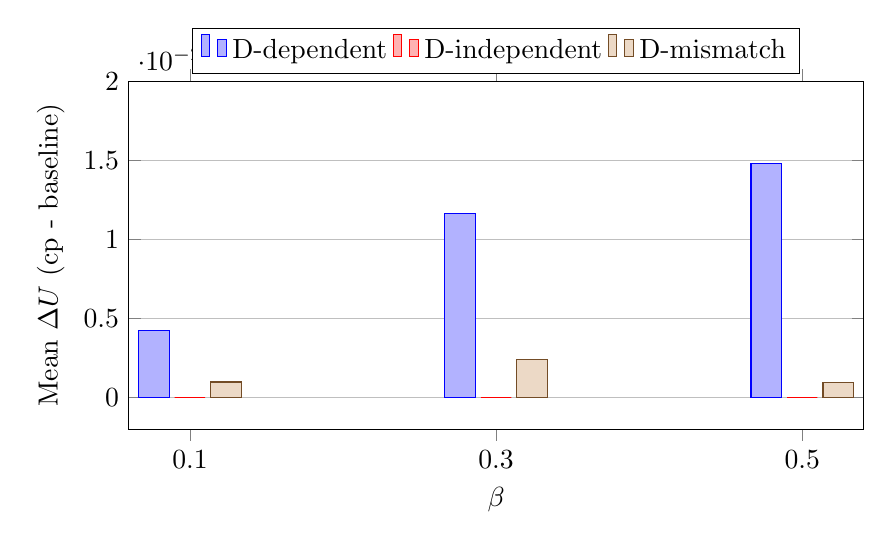
\begin{tikzpicture}
\begin{axis}[
    ybar,
    bar width=11pt,
    width=0.9\textwidth,
    height=6.0cm,
    xlabel={$\beta$},
    ylabel={Mean $\Delta U$ (cp - baseline)},
    symbolic x coords={0.1,0.3,0.5},
    xtick=data,
    legend style={at={(0.5,1.02)},anchor=south,legend columns=3},
    ymin=-0.002, ymax=0.02,
    ymajorgrids=true
]
\addplot coordinates {(0.1,0.004259) (0.3,0.011637) (0.5,0.014776)};
\addplot coordinates {(0.1,0.000000) (0.3,0.000000) (0.5,0.000000)};
\addplot coordinates {(0.1,0.000983) (0.3,0.002380) (0.5,0.000950)};
\legend{D-dependent,D-independent,D-mismatch}
\end{axis}
\end{tikzpicture}
\caption{Mean utility difference by dependency condition and coupling gain.}
\label{fig:udiff}
\end{figure}

\subsection{Independent-equivalence check}
For all 9 D-independent runs (3 patterns $\times$ 3 beta levels),
\(\max|w^{\mathrm{cp}}-w^{\mathrm{base}}|=0.0\), satisfying the tolerance criterion.

\subsection{Pass/fail outcomes}
From `cp\_v2\_report.json`:
\begin{itemize}
  \item C1: pass (D-dependent mean \(\Delta U\) at \(\beta=0.3\) is 0.0116)
  \item C2: pass (D-independent mean \(\Delta U\) at \(\beta=0.3\) is 0.0000)
  \item C3: fail (D-dependent oscillation rate mean at \(\beta=0.3\) is 0.5355)
  \item C4: pass (all independent-equivalence checks true)
\end{itemize}
This run therefore rejects unconditional cp advantage and indicates a stability tradeoff under the current operator streams.

\section{Applicability and Failure Conditions}
cp is applicable when candidate dependencies are bounded and interpretable, and when directional updates (\(\sigma/\delta\)) remain sufficient.

Failure modes to report explicitly:
\begin{enumerate}
  \item oscillation escalation under coupling,
  \item over-coupling collapse (mass concentration),
  \item mismatch sensitivity when dependency signs are wrong,
  \item interface parse break for \((\sigma/\delta,\text{target})\).
\end{enumerate}
For (3) or (4), set `TRANSFER\_PRINCIPLES\_REEVAL\_REQUIRED=true` and continue cp-side analysis.

\section{Reproducibility}
Implementation and steps:
\begin{itemize}
  \item `spec/nrr-coupled\_spec\_v2.md`
  \item `repro/coupled\_state\_sim.py`
  \item `repro/README\_v2.md`
\end{itemize}
No API calls are required in the main protocol.

\section{Conclusion}
cp extends Transfer with deterministic dependency propagation while preserving the LLM interface contract. In this simulation-first evaluation, cp provides small utility gains in dependency-present settings and exact equivalence under independence, but increases oscillation under tested streams. The evidence supports conditional, not universal, usefulness.

\begin{thebibliography}{9}
\bibitem{saito2025nrr}
Saito, K. (2025).
\textit{NRR-Core: Non-Resolution Reasoning as a Computational Framework for Contextual Identity and Ambiguity Preservation}.
arXiv:2512.13478.

\bibitem{saito2026phi}
Saito, K. (2026).
\textit{NRR-Phi: Text-to-State Mapping for Ambiguity Preservation in LLM Inference}.
arXiv:2601.19933.

\bibitem{saito2026transfer}
Saito, K. (2026).
\textit{NRR-Transfer: Cross-Domain Transfer of Phase 1.5 Operators Under Fixed Interface Constraints}.
Manuscript v30 (pre-submission line).
\end{thebibliography}

\end{document}
